\documentclass[a4paper, 11pt]{article}
\usepackage{fullpage}
\usepackage{indentfirst}
\usepackage{graphicx}
\usepackage{amsmath}
\usepackage{algorithm}
\usepackage[noend]{algpseudocode}
\usepackage{verbatim}
\usepackage{url}
\usepackage[justification=centering]{caption}
\title{\vspace{-2cm}\huge Phase Synchronization Capability of \\TwinRX Daughterboards and DoA Estimation}

\begin{document}
\date{\vspace{-5ex}}
\maketitle
\date{\vspace{-5ex}}
\section*{\underline{Introduction}}
This article will provide instructions for demonstrating the phase synchronization capability of Ettus Research's TwinRX daughtercards. TwinRX daughtercards can achieve a high degree of accurate phase synchronization except for constant repeatable relative phase offsets. In this article, we will demonstrate a simple method to determine the accuracy of phase synchronization achieved followed by an application of great practical importance in modern wireless communications which fundamentally relies on accurate phase synchronization. 

\section*{\underline{Motivation}}
Ettus Research$^{\mathrm{TM}}$ provides several convenient solutions for synchronization across multiple USRP$^{\mathrm{TM}}$ (Universal Software Radio Peripheral) devices, which is a critical requirement for certain applications. See~\cite{pandeya} for detailed instructions. The easiest method to implement a basic high-performance 2x2 MIMO system is to utilize two N200/N210s synchronized with an Ettus Research MIMO cable. In this configuration, the USRP connected to the GigE acts as a switch and routes data to/from both USRP devices. It will also handle time synchronization of the data so the sample alignment process is transparent to the user.

It is also possible to synchronize multiple devices using external 10 MHz and 1 PPS distribution. The Ettus Research OctoClock and OctoClock-G make it easy to distribute 10 MHz and 1 PPS signals for multi-channel operation. The OctoClock serves as an 8-way PPS and 10 MHz reference splitter. The user must provide a single 10 MHz and 1 PPS signal. The upgraded OctoClock-G includes a high-accuracy, internal GPS-disciplined oscillator and does not require external signals to be supplied. Figure~\ref{octoclock_sync} illustrates the use of an OctoClock to create a 4x4 MIMO system. All timing signals from the OctoClock should be connected to the USRP devices with matched length cable of the same type and connectorization. This ensures that there is low skew between all of the channels. 
\begin{figure}[t]
    \centering
    \includegraphics[width=0.8\textwidth]{figures/octoclock_mimo.pdf}
    \caption{Synchronizing Multiple USRPs using an Octoclock.}
    \label{octoclock_sync}
\end{figure}
\begin{figure}[h!]
    \centering
    \includegraphics[width=0.8\textwidth]{figures/phase_correct_image.png}
    \caption{A Photograph of the Experimental Setup for TwinRX Relative Phase Offset Measurement and Correction.}
    \label{twinrx_phase_correct_image}
\end{figure}

In addition to the methods outlined above, Ettus Research has introduced the TwinRX daughterboard for USRP X Series radios which is a dual channel superheterodyne receiver that offers a wide dynamic range and accurate phase synchronization except for constant repeatable relative phase offsets. It is achieved by the ability to share the LO between channels across two TwinRX daughterboards within an X Series radio. This enables phase-aligned operation required to implement four-channel phased arrays. In other words, with a radio configuration consisting of a USRP X300/X310 installed with two TwinRXs, the user has access to four synchronized receive channels without requiring an OctoClock. 

\section*{\underline{Phase Offset Measurement and Correction}}
As we mentioned previously, a USRP X310 equipped with TwinRX daughterboards is capable of sharing LOs and clock/time references. The relative phase-offsets between the receive channels are repeatable constant values across runs which need to be estimated as a first step. For this step, we will need:
\begin{itemize}
\item 1 USRP X310 with two TwinRXs installed.
\item 1 USRP N210 with an SBX daughterboard (or another USRP/daughterboard of your choice) which will function as a transmitter\footnotemark\footnotetext{Although we used a USRP as the transmitter, any RF test equipment such as a signal generator which can transmit a tone while satisfying the operational specifications of X310/TwinRX can also be used.}.
\item 5 SMA-M to SMA-M cables. 4 of these need to be of equal length.
\item 1 four-way power splitter (e.g., Mini-Circuits ZFRSC-4-842+).
\item 1 30 dB attenuator.
\end{itemize}
The setup required to calibrate the X310 with two TwinRXs for phase-alignment is shown in Figure~\ref{twinrx_phase_correct_image}. Connect the transmitter to the four receive ports on the X310 via an attenuator and a power splitter. Use four equal-length cables to connect the output ports of the power splitter to the input ports of the X310. We will then transmit a tone (e.g., of frequency 10 KHz). To do so, in the host PC connected to the transmitter USRP, navigate to the \texttt{gr-doa/apps} directory and open the flowgraph titled, \texttt{run\_DoA\_transmitter.grc}. The user-defined variables are contained in the \texttt{struct} variable titled, \texttt{input\_variables}. Here, select appropriate values for parameters such as tone frequency, sample rate, center frequency, ip-address of the device and transmit gain based on the USRP/daughterboard combination of your transmitter. Then, in the host PC connected to the receive X310, open the flowgraph titled, \texttt{estimate\_X310\_TwinRX\_constant\_phase\_offsets\_and\_save.grc}. Ensure that the tone frequency, sample rate and center frequency are the same as those used at the transmitter. Provide the ip-address of the X310 device. The config filename that contains the measured constant relative phase offsets is also customizable. A screenshot of the flowgraph is shown in Figure~\ref{twinrx_phase_est_flowgraph}. Now, execute the flowgraph. 
\begin{figure}[t]
    \centering
    \includegraphics[width=0.8\textwidth]{figures/measure_phase_offsets.png}
    \caption{TwinRX Relative Phase Offset Estimation Flowgraph.}
    \label{twinrx_phase_est_flowgraph}
\end{figure}
\begin{figure}[hb!]
    \centering
    \includegraphics[width=0.8\textwidth]{figures/Time_Sink_GUI_View_X310_TwinRX_output_with_corrected_phase_offsets.png}
    \caption{Time Domain Display Showing Received Signal with
Phase Compensation.}
    \label{time_gui_phase_comp}
\end{figure}

The output of the X310 with compensated relative phase offsets can be observed by running \texttt{view\_X310\_TwinRX\_op\_with\_corrected\_phase\_offsets.grc} flowgraph in the \texttt{apps} directory. Ensure that the parameters selected are the same as those used for measuring the offsets. Observe that the time-scope display is similar to that shown in Figure~\ref{time_gui_phase_comp}. The accuracy of the phase offset compensation can also be saved in a numerical format by executing the flowgraph, \texttt{calculate\_X310\_TwinRX\_phase\_sync\_accuracy.grc}. In our experiments, we observed that phase misalignment between the four streams is less than $0.5$ degrees regardless of the particular combination of center frequency, tone frequency and sample rate. 

However, this calibration is valid for a particular choice of center frequency, tone frequency and sample rate only. The phase offset measurement and correction step needs to be repeated when these operating parameters are modified. As a result of this calibration step, the relative phase offsets observed between the four streams when receiving signals across an antenna-array will be a function of the \textit{array-manifold} alone. Any user-developed array signal processing application that requires accurate phase synchronization between receive channels will need to incorporate this compensation step as the first stage of processing. To demonstrate how this is done, we will show two direction-of-arrival (DoA) estimation algorithms in action. 

\section*{\underline{Signal and Noise Subspaces}}
First, we look at a brief theoretical overview of signal and noise subspaces. Subspace methods are widely used for DoA estimation and rely on exploiting the orthogonality between signal and noise subspaces. For detailed background, see~\cite{trees}. Suppose that an antenna array is composed of $N$ isotropic sensors which are located at positions, $p_n$ for $n\in\{0,\,1,\,...,N-1\}$. Suppose that $x(t)$ is the signal received by the antenna array and it consists of $D$ directional plane-wave processes plus white sensor noise. That is, 
\begin{equation*}
x(t) = \sum_{d=1}^{D}\tilde{f}_d(t)\,\mathbf{v}(\mathbf{k}_d)+w(t). 
\end{equation*}
where, $\mathbf{v}(\mathbf{k})$ is the \textit{array manifold vector},
\begin{equation}
\mathbf{v(k)}=\left[e^{-j\mathbf{k}^T p_0}\quad e^{-j\mathbf{k}^T p_1}\hdots\quad e^{-j\mathbf{k}^T p_{N-1}}\right]^T
\label{amv}
\end{equation}
evaluated for the specific \textit{wave number}\footnotemark\footnotetext{The \textbf{wavenumber}, $\mathbf{k}$ for a plane wave as:
\begin{equation*}
\mathbf{k} = -\frac{\Omega}{c}\mathbf{u} = -\frac{2\pi}{\lambda}\mathbf{u} = -\frac{2\pi}{\lambda}\left[\sin(\theta)\cos(\phi) \:\:\: \sin(\theta)\sin(\phi) \:\:\: \cos(\theta)\right]^T,
\end{equation*} where, $\mathbf{u}$ is the directional cosines vector.}, $\mathbf{k}_d$ associated with the $d$th target. Suppose that $\tilde{f}_d(t)$, for $d=1,2,\hdots,D$, is bandlimited to $W$ and we sample $x(t)$ every $1/W$ seconds to obtain a discrete-time domain snapshot model. By denoting the snapshots as $\mathbf{x}(k)$, for $k=1,2,\hdots,K$, we can write the correlation matrix of the input streams as follows:
\begin{equation}
\mathbf{R}_{\mathbf{x}}(k) = E\left[\mathbf{x}(k)\,\mathbf{x}^H(k)\right] = \mathbf{V}\mathbf{R_f}\mathbf{V}^H+\sigma_w^2\,\mathbf{I}. 
\label{cov_mat1}
\end{equation}
In practice, we construct a \textit{sample} correlation matrix as an estimate for the true autocorrelation matrix. The method chosen for constructing the sample correlation matrix influences the performance of the DoA estimators. One approach to constructing a sample correlation matrix is to collect a sample during each time snapshot, across $N$ array elements into a $N\times 1$ vector $\mathbf{x}(k)$, and perform the following operation:
\begin{equation}
\mathbf{C_x} = \frac{1}{K}\sum_{k=1}^{K}\mathbf{x}(k)\,\mathbf{x}^H(k).
\end{equation}
where, $K$ is the number of snapshots. An alternative way of computing this sample correlation matrix is to collect samples across several time snapshots, into a $N\times K$ matrix $\mathbf{X_k}$, and perform the following operation:
\begin{equation}
\mathbf{C_x} = \frac{1}{K}\mathbf{X_K}\,\mathbf{X_K}^H.
\end{equation}
It has been argued that performing an additional Forward-Backward Averaging step in determining the sample correlation matrix will result in superior DoA estimator performance~\cite{trees}. It can be written as follows, 
\begin{align}
\mathbf{C_x} &= \frac{1}{2K}\mathbf{X_K}\,\mathbf{X_K}^H+\frac{1}{2K}\,\mathbf{J}\,\mathbf{X_K}^*\,\mathbf{X_K}^T\,\mathbf{J}.
\end{align}
where, $\mathbf{J}$ is a square $N\times N$ \textit{reflection matrix} whose elements on the cross diagonal are unity and all other elements are zero. Similar to \eqref{cov_mat1}, we can write the sample correlation matrix as follows: 
\begin{equation}
\mathbf{C_x} = \mathbf{V}\mathbf{R_f}\mathbf{V}^H+\sigma_w^2\,\mathbf{I}. 
\label{cov_mat2}
\end{equation}
An important assumption implicit in the subspace methods for DoA estimation is that no two of the $D$ signals are coherent, \textit{i.e.}, $\mathbf{R_f}$ is positive definite. In \eqref{cov_mat1} and \eqref{cov_mat2}, we defined the $N\times D$ \textit{array manifold matrix}, $\mathbf{V}$\footnotemark\footnotetext{For a uniform linear array, assuming the locations of the antenna elements to be:
\begin{equation*}
p_{x_n} = 0,\:\:p_{y_n} = 0,\:\:p_{z_n} = \left(n-\frac{N-1}{2}\right)\,d,\qquad\quad n=0,\,1,\,\hdots,\,N-1,
\end{equation*} we can show that
\begin{equation*}
\mathbf{v}(k_z)=\left[e^{j\left(\frac{N-1}{2}\right)k_z d}\quad e^{j\left(\frac{N-3}{2}\right)k_z d}\quad\hdots\quad e^{-j\left(\frac{N-1}{2}\right)k_z d}\right]^T,
\end{equation*}
where, $k_z = -\frac{2\pi}{\lambda}\cos(\theta)$. It is helpful to also define, $\psi = -k_z\,d$.} as follows:
\begin{equation}
\mathbf{V}:=\left[\mathbf{v}(\mathbf{k}_1)\quad \mathbf{v}(\mathbf{k}_2)\quad\hdots\quad \mathbf{v}(\mathbf{k}_D)\right]^T.
\label{amm}
\end{equation}
The columns of $\mathbf{V}$ span a $D$-dimensional subspace that contains all of the signal energy. We can obtain the orthogonal basis of this subspace, $\{\Phi_d\}$ for $d=1,2,\hdots,D$ as follows. The first step is to recognize that $\Phi_d$ is the linear transformation, $\Phi_d = \mathbf{V c}_d$ for some $D\times 1$-vector, $\mathbf{c}_d$. Now, the eigenvalue decomposition (EVD) of the first term in \eqref{cov_mat2} is:
\begin{align}
& \lambda\Phi_d = \mathbf{V}\mathbf{R_f}\mathbf{V}^H\Phi_d \nonumber \\
\Rightarrow& \lambda\mathbf{V c}_d = \mathbf{V}\mathbf{R_f}\mathbf{V}^H\mathbf{V c}_d \nonumber \\
\Rightarrow& \mathbf{V}\left[\lambda\mathbf{I}-\mathbf{R_f}\mathbf{V}^H\mathbf{V}\right]\mathbf{c}_d = \mathbf{0}. \nonumber
\end{align}
The above condition is met by the $D$ solutions, $\lambda_1^s\geq \lambda_2^s\geq \hdots \geq \lambda_D^s$ of 
\begin{equation*}
\mathrm{det}\left(\lambda\mathbf{I}-\mathbf{R_f}\mathbf{V}^H\mathbf{V}\right) = 0.
\end{equation*}
That is, we perform the EVD of $\mathbf{R_f}\mathbf{V}^H\mathbf{V}$. The corresponding eigenvectors, $\mathbf{c}_d$ are used to obtain the orthogonal basis, $\{\Phi_d\}$ for $d=1,2,\hdots,D$. We can now form the $N\times D$ matrix, 
\begin{equation}
\mathbf{U}_S := \left[\Phi_1\quad\Phi_2\quad\hdots\quad\Phi_D\right].
\end{equation}
The range space of $\mathbf{U}_S$ is referred to as the \textbf{signal subspace}. On the other hand, referring to \eqref{cov_mat2}, we notice that the noise component spans the entire $N$-dimensional space. Consequently, we need $(N-D)$ additional orthogonal vectors to represent it. Any arbitrary set of vectors that are orthogonal to each other and orthogonal to $\mathbf{U}_S$ meet the requirement. We now form the $N\times (N-D)$ matrix, 
\begin{equation}
\mathbf{U}_N := \left[\Phi_{D+1}\quad\Phi_{D+2}\quad\hdots\quad\Phi_N\right].
\end{equation}
The range space of $\mathbf{U}_N$ is referred to as the \textbf{noise subspace}. In summary,
\begin{equation}
\mathbf{C_x} = \sum_{n=1}^{N}\lambda_n\Phi_n\Phi_n^H,
\end{equation}
where,
\begin{equation}
\lambda_n=
\begin{cases}
\lambda_n^s+\sigma_w^2, & \text{if}\ n=1,2,\hdots,D \\
\sigma_w^2, & \text{if}\ n=D+1,D+2,\hdots,N. 
\end{cases}
\end{equation}
Alternatively, by defining the $D\times D$ diagonal matrix, $\Lambda_S := \mathrm{diag}\left[\lambda_1,\,\lambda_2,\,\hdots,\,\lambda_D\right]$ and the $(N-D)\times(N-D)$ diagonal matrix, $\Lambda_N=\sigma_w^2\mathbf{I}$, we can write, 
\begin{equation}
\mathbf{C_x} = \mathbf{U}_S\Lambda_S\mathbf{U}_S^H+\mathbf{U}_N\Lambda_N\mathbf{U}_N^H.
\end{equation}
This idea of decoupling the signal subspace from its orthogonal noise subspace is fundamental to many array processing methods.

\section*{\underline{MUSIC and Root-MUSIC Algorithms}}
The discussion we have seen so far is the basis for several subspace-based methods. One of the earliest algorithms within the family of subspace methods for DoA estimation is Multiple Signal Classification (MUSIC). MUSIC requires that the following assumptions are satisfied: (1) the received waveform is narrowband, (2) the received waveform consists of $D$ plane-wave signals plus \textit{uncorrelated} noise, (3) the \textit{number} of plane-wave signals, $D$ is known (4) the number of antenna elements, $N$ is at least equal to $D+1$. A summary of MUSIC for linear arrays is as follows:
\begin{algorithm}[H]
\renewcommand{\thealgorithm}{}
\begin{algorithmic}[1]
\State \text{Construct the \textit{sample} correlation matrix, $\mathbf{C_x}$.}
\State \text{Determine $\mathbf{U_N}$, the noise subspace from $\mathbf{C_x}$ using Eigen-Value Decomposition (EVD).}
\For{$0\leq\theta\leq \pi$ \text{(alternatively, $-\frac{2\pi\,d}{\lambda}\leq\psi\leq \frac{2\pi\,d}{\lambda}$)}}
\State Generate the corresponding array manifold vector, $\mathbf{v}(\psi)$.  
\State Compute the \textit{null-spectrum}, \label{null_spectrum_line}
\Statex $\phantom{indentation}$ $Q(\psi) := ||\mathbf{v}^H(\psi)\mathbf{U_N}||^2 = \mathbf{v}^H(\psi)\mathbf{U_N}\mathbf{U}^H_\mathbf{N}\mathbf{v}(\psi)$.
\EndFor
\State Choose the $D$ minima of $Q(\psi)$. The corresponding values of $\psi$ are the $D$ angles of arrival. 
\end{algorithmic}
\caption{MUSIC}
\end{algorithm}
It can be noticed from line~\ref{null_spectrum_line} of the above algorithm that whenever $\psi$ equals the true angle of arrival, $Q(\psi)$ equals zero since $\mathbf{v}(\psi)$ will be a basis vector of the signal subspace and is therefore, orthogonal to the noise subspace. This is the underlying principle behind MUSIC algorithm. For visualization purposes, it is a common practice to plot $1/Q(\psi)$, termed \textit{pseudo-spectrum}. 

Root MUSIC is a straight-forward variant of MUSIC algorithm which involves finding the roots of a polynomial instead of plotting the pseudospectrum across all values of the polar angle, $\theta$ and searching for the peaks. Consider a Uniform Linear Array whose array manifold vector is written as,
\begin{equation}
\mathbf{v}(\psi)=e^{-j\left(\frac{N-1}{2}\right)\psi}\left[1\quad e^{j\psi}\hdots\quad e^{j(N-1)\psi}\right]^T.
\end{equation}
An equivalent phase-shifted representation is,
\begin{equation}
\mathbf{v}(z)=\left[1\quad z\quad\hdots\quad z^{N-1}\right]^T.
\end{equation}
It is easy to verify that, $\mathbf{v}(z)|_{z = e^{j\psi}}=e^{j\left(\frac{N-1}{2}\right)\psi}\mathbf{v}(\psi)$. Now, a polynomial representation of the null-spectrum is, 
\begin{align}
Q(z) &= \mathbf{v}^T(1/z)\mathbf{U_N}\mathbf{U}^H_\mathbf{N}\mathbf{v}(z) \nonumber \\
& \stackrel{\text{(a)}}{=} \sum_{m=0}^{N-1}\sum_{n=0}^{N-1}z^{-m}\,\mathbf{U}^2_\mathbf{N}(m, n)\,z^{n} \nonumber \\
& \stackrel{\text{(b)}}{=} \sum_{-N+1}^{\phantom{+}N-1}u_l\,z^l.
\label{rMUSIC_poly_eq}
\end{align}
In (a), we defined the ``square'' of $\mathbf{U_N}$ as $\mathbf{U}^2_\mathbf{N}:=\mathbf{U_N}\mathbf{U}^H_\mathbf{N}$. In (b), for $l>0$, $u_l$ is the sum of elements along the $l$th super-diagonal and for $l<0$,  $u_l$ is the sum of elements along the $l$th sub-diagonal. Clearly, $\mathbf{U}^2_\mathbf{N}$ is a Hermitian non-negative definite matrix and the relation, $u_l = u^*_{-l}$ holds true. Due to this result, we need to compute only $N-1$ polynomial coefficients. Notice that plotting the null-spectrum, $Q(\psi)$ and choosing $D$ minima is equivalent to finding $D$ out of $2(N-1)$ roots of $Q(z)$ that lie on the unit circle. In practice, due to the presence of noise, the roots will not necessarily be on the unit circle. So, we choose the $D$ roots that are inside the unit circle and closest to the unit circle. We can now summarize Root-MUSIC as follows:
\begin{algorithm}[H]
\renewcommand{\thealgorithm}{}
\begin{algorithmic}[1]
\State Construct the \textit{sample} correlation matrix, $\mathbf{C_x}$.
\State Determine $\mathbf{U_N}^2$, the ``square'' of noise subspace from $\mathbf{C_x}$ using Eigen-Value Decomposition (EVD).
\State Determine the roots of the polynomial, $Q(z)=\sum_{-N+1}^{\phantom{+}N-1}u_lz^l$. For $l>0$, $u_l$ is the sum of elements of $\mathbf{U_N}^2$ along the $l$th super-diagonal and for $l<0$,  $u_l$ is the sum of elements of $\mathbf{U_N}^2$ along the $l$th sub-diagonal. 
\State Choose $D$ roots, $\{z_d\}$ for $d=1,2,\hdots,D$ that are inside the unit circle and closest to the unit circle.
\State Obtain $\{\theta_d\}$ for $d=1,2,\hdots,D$ using the relation,
\Statex $\phantom{indentation}$ $\theta_d=\mathrm{acos}\left(\,\mathrm{arg}(z_d)\times\lambda/(2\pi d)\,\right)$.
\end{algorithmic}
\caption{Root MUSIC}
\end{algorithm}
It must be noted that unlike MUSIC algorithm, Root-MUSIC is not generalizable for arbitrary array geometries. Consequently, the current implementation of Root-MUSIC in \texttt{gr-doa} supports linear array geometry only.

\subsection*{Simulation Examples}
A GNU Octave based simulation testbench is available in the \texttt{@wpi\_twinrx\_doa\_testbench} directory under \texttt{gr-doa/examples} that implements MUSIC algorithm for DoA estimation. To list the arguments needed to create the simulation testbench, open Octave and at the command-prompt, type \texttt{help doa\_testbench\_create}. For a  demonstration of DoA estimation using MUSIC algorithm for linear arrays, run the script, \texttt{estimate\_doa\_MUSIC\_linear\_array.m}. A Pseudo-Spectrum plot is shown in Figure~\ref{music_sim} for a simulation setting involving targets present at angles, $30^o$ and $125^o$. Simulation flowgraphs that utilize blocks developed using GNU Radio framework for implementing MUSIC are available in \texttt{gr-doa/apps}.
\begin{figure}[t]
    \centering
    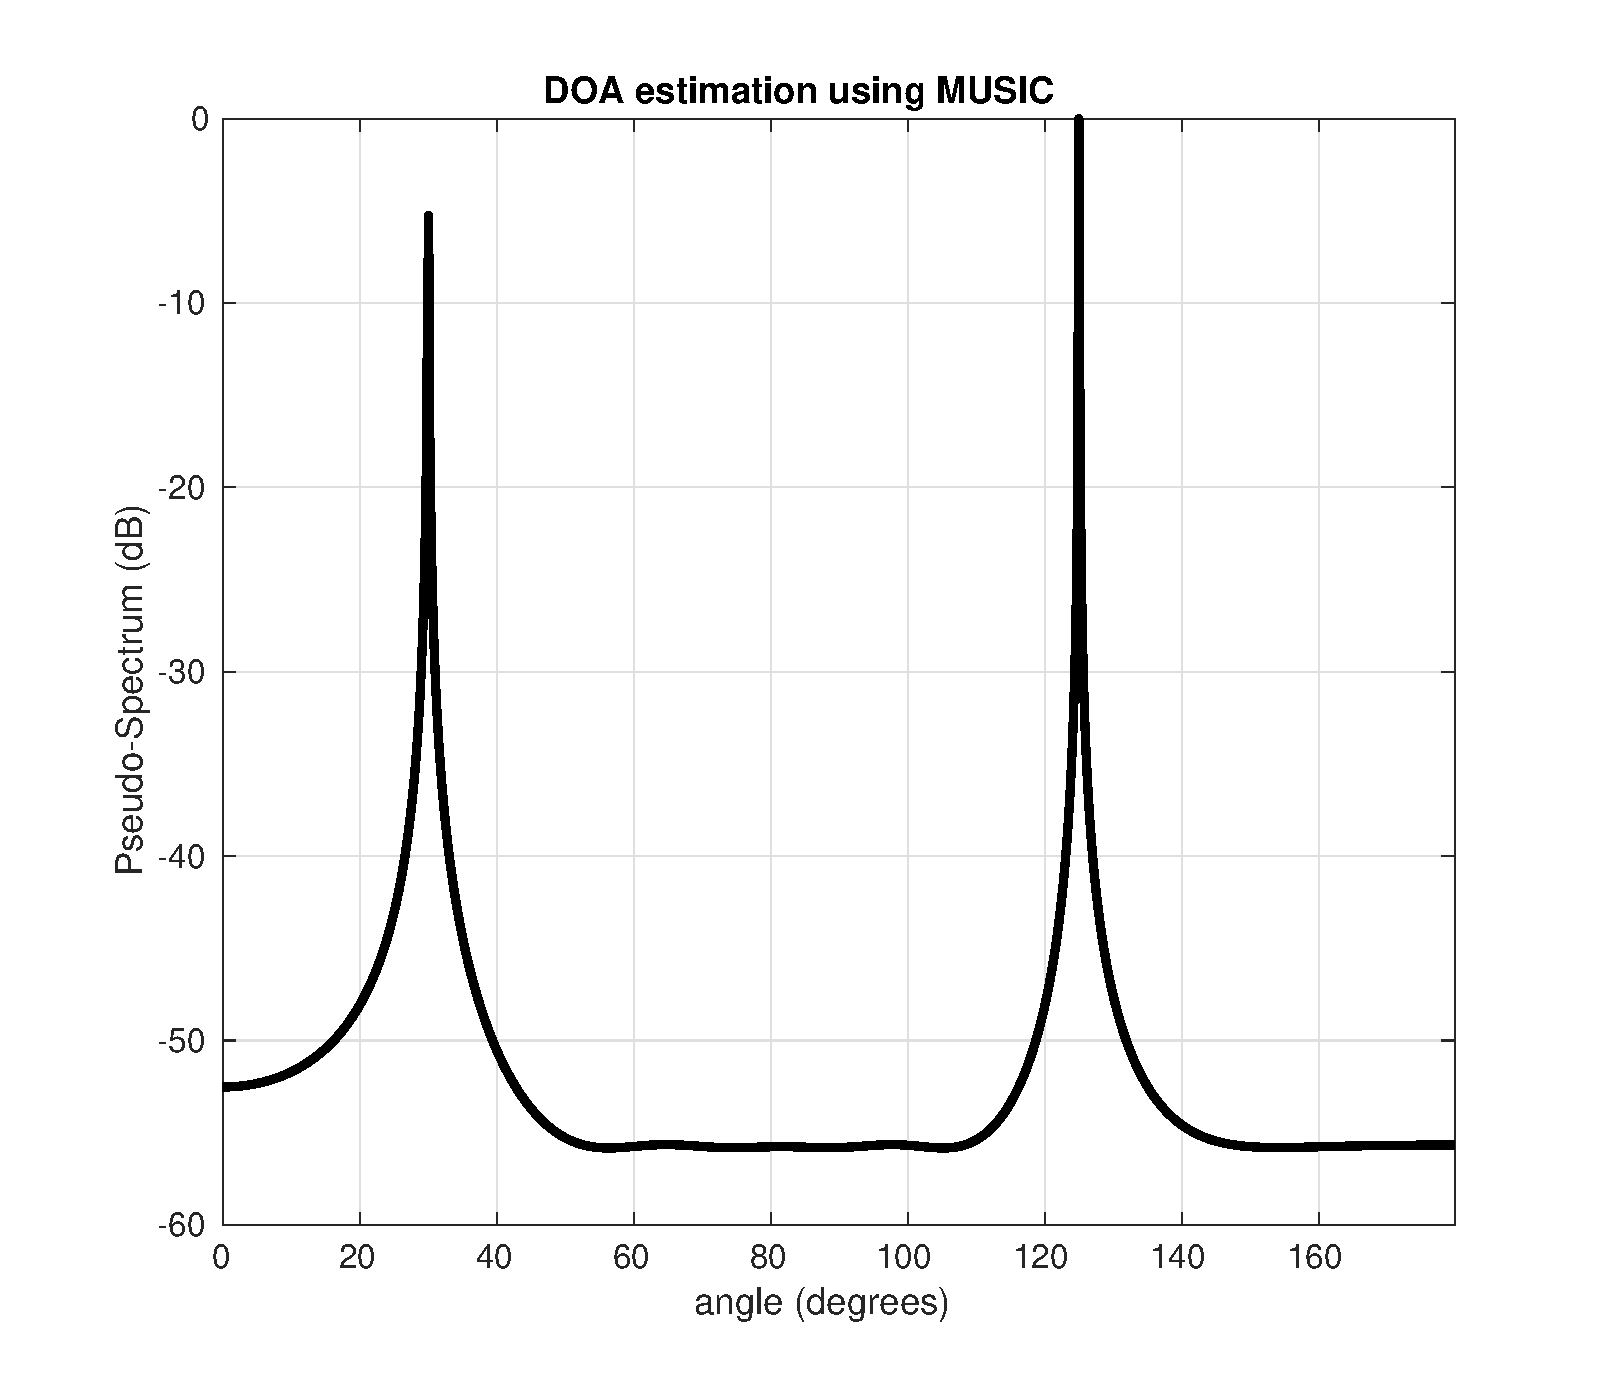
\includegraphics[width=0.6\textwidth]{figures/MUSIC_lin_array_sim.eps}
    \caption{Pseudo-Spectrum of a Simulated 2-target DoA Estimation Scenario.}
    \label{music_sim}
\end{figure}

The GNU Octave based simulation testbench, \texttt{wpi\_twinrx\_doa\_testbench} also contains an implementation of Root-MUSIC algorithm for DoA estimation. To run a simulation example that demonstrates DoA estimation using Root-MUSIC algorithm for linear arrays, run the script, \texttt{estimate\_doa\_RootMUSIC\_linear\_array.m}. Since Root-MUSIC algorithm generates roots of a polynomial, it does not have an associated visual representation. However, by running the simulation flowgraph, \texttt{gr-doa/apps/run\_RootMUSIC\_lin\_array\_simulation.grc}, the resultant polynomial roots can be seen on a compass display. 

\section*{\underline{Physical Experiments using a USRP X310 with 2 TwinRXs}}
We now discuss the methodology involved in performing DoA estimation with the blocks developed using GNU Radio framework. In addition to the list of items indicated previously, we also require:
\begin{itemize}
\item 5 Vert2450 antennas (or other antennas of your choice which have a good gain-phase relationship in your frequency band of choice). 
\item (Optional) An array fixture with variable antenna element spacing and 4 equal length SMA-M to SMA-M cables to connect the antennas held in place by the array fixture to the TX/RX and RX2 ports of RF-A and RF-B on the X310.
\end{itemize}
\textbf{NOTE}: It is strongly recommended that the antenna element separation is half-wavelength or lower depending on the tone center-frequency. Arranging antenna elements at larger distances leads to an aliasing effect and compromises the angle resolution capability of the DoA algorithms. 

Disconnect the cables connecting the transmitter and the receiver. Position the transmitter at a distance in the far-field from the receiver antenna array. Note the geometrical angle that is to be expected. At this point, we assume that the user has performed the relative phase offset measurement and correction stage as outlined previously. In the host PC that is connected to the transmitter USRP, navigate to the \texttt{gr-doa/apps} directory and open the flowgraph titled, \texttt{run\_DoA\_transmitter.grc}. The user-defined variables are contained in the \texttt{struct} variable titled, \texttt{input\_variables}. Here, select appropriate values for parameters such as tone frequency, sample rate, center frequency, ip-address of the device and transmit gain based on the USRP/daughterboard combination of your transmitter. 
\begin{figure}[b!]
    \centering
    \includegraphics[width=0.95\textwidth]{figures/MUSIC_lin_flowgraph.png}
    \caption{MUSIC DoA Estimation Flowgraph for Linear Antenna Arrays.}
    \label{MUSIC_doa_est_lin}
\end{figure}
\begin{figure}[t!]
    \centering
    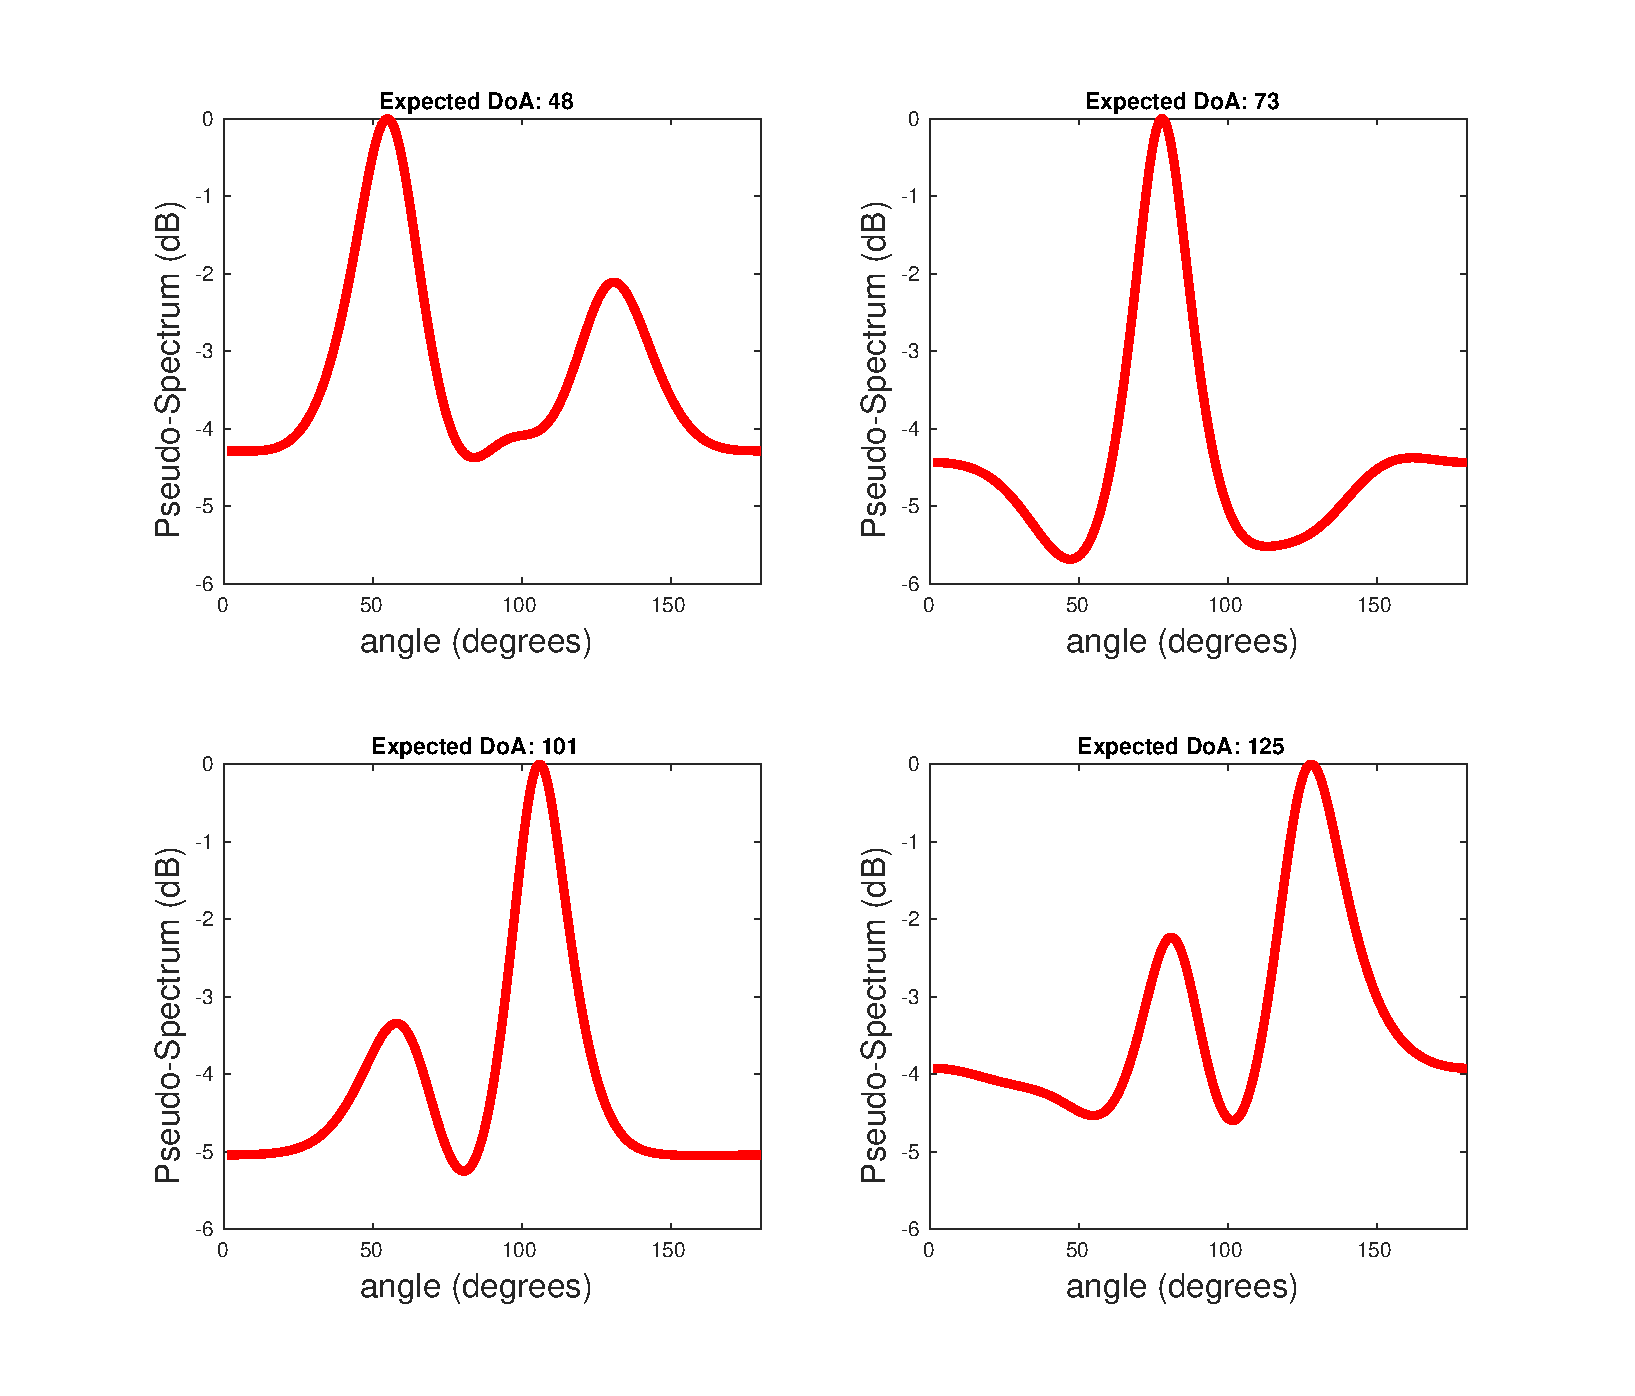
\includegraphics[width=0.85\textwidth]{figures/MUSIC_lin_array_X310_1target.eps}
    \caption{Pseudo-Spectrum of a 1-target DoA Estimation Scenario using a Linear Array.\\ Experiments Conducted in an Anechoic Chamber.}
    \label{music_x310}
\end{figure}

Now, assuming that a linear antenna array is being used for DoA estimation, navigate to the \texttt{gr-doa/apps} directory in the host PC that is connected to the receiver USRP and open the flowgraph titled, \texttt{run\_MUSIC\_lin\_array\_X310\_TwinRX.grc}. Again, select appropriate values for the ip-address of the receiver, receive gain, number of array elements, normalized spacing of the antenna elements etc. Ensure that parameters such as tone frequency, sample rate and center frequency are the same as those selected at the transmitter. Ensure that the correct config file for phase offset correction is selected in the \texttt{Phase Correct} block. A screenshot of the this flowgraph is shown in Figure~\ref{MUSIC_doa_est_lin}. Execute this flowgraph to see DoA estimation performance over a linear array. 

We now discuss our DoA estimation results using the flowgraph mentioned above. We used a USRP N210 as the transmitter and a calibrated USRP X310 with 2 TwinRXs as the receiver. The experiments were conducted in an anechoic chamber of approximate dimensions, $3~\mathrm{m(L)}\times 2~\mathrm{m(W)}\times 3~\mathrm{m(H)}$. We conducted this experiment for a range of transmitter positions with respect to the receiver. In Figure~\ref{music_x310}, we show the performance of MUSIC in terms of the Pseudo-Spectrum for four directions of arrival. Despite the fact that we conducted measurements in a reasonably controlled environment, as shown in this figure, we occasionally observed strong secondary peaks which were nevertheless weaker compared to the peak corresponding to the true direction of arrival. In these experiments, the spacing between the antenna elements was $1$~\textit{in} and the center frequency was selected such that this spacing corresponded to half-wavelength of the carrier. The sample rate chosen was $1$~MS/s. 

\subsection*{Effect of Antenna Calibration on DoA Estimation}
Based on Figure~\ref{music_x310}, we noticed that the SNR of the pseudo-spectrum is rather low despite conducting experiments in a reasonably ideal environment. While relative phase offset correction across the receive streams is one aspect of the overall calibration process, we demonstrate in this subsection that calibrating the antenna element gains and phases also has a noticeable effect. To do so, we provide a brief overview of the approach adopted based on~\cite{soon1994}. 

Suppose that $\Gamma := \mathrm{diag}\{1,\;\alpha_1 e^{-j\theta_1},\hdots,\alpha_{N-1} e^{-j\theta_{N-1}}\}$ represents the diagonal matrix consisting of the non-uniform antenna gains and phases along its principal diagonal. It can be showed that this effect can be captured by updating \eqref{cov_mat2} as shown below:
\begin{equation}
\mathbf{C_x} = \Gamma\,\mathbf{V}\mathbf{R_f}\mathbf{V}^H\Gamma^H+\sigma_w^2\,\mathbf{I}. 
\label{cov_mat_ant}
\end{equation}
Now, taking the EVD of $\mathbf{C_x}$ gives,
\begin{equation}
\mathbf{C_x} = \mathbf{E}_S\Lambda_S\mathbf{E}_S^H+\sigma_w^2\,\mathbf{E}_N\mathbf{E}_N^H.
\end{equation}
where, $\mathbf{E}_S$ denotes the eigenvector matrix of $\mathbf{C_x}$ associated with the signal subspace spanned by $\Gamma\,\mathbf{V}$. Thus, the solution set of sensor gains and phases and directions of arrival are constrained such that 
\begin{equation*}
\mathbf{E}_S\mathbf{E}_S^H\Gamma\,\mathbf{V} = \Gamma\,\mathbf{V}.
\end{equation*}
Equivalently, 
\begin{equation*}
\mathbf{E}_S\mathbf{E}_S^H\Gamma\,\mathbf{v(k_d)} = \Gamma\,\mathbf{v(k_d)},\qquad d = 1,\hdots,D. 
\end{equation*}
By defining $\mathbf{V_d}=\mathrm{diag}(\mathbf{v(k_d)})$ and $\gamma = [1,\;\alpha_1 e^{-j\theta_1},\hdots,\alpha_{N-1} e^{-j\theta_{N-1}}]^T$, the above equation becomes, 
\begin{equation*}
\mathbf{E}_S\mathbf{E}_S^H\mathbf{V_d}\,\gamma = \gamma\,\mathbf{V_d}\qquad d = 1,\hdots,D. 
\end{equation*}
Since $\mathbf{V_d}$ is a diagonal matrix composed entirely of the array-manifold vector, it is also unitary. Hence,  
\begin{equation*}
\mathbf{V_d}^H\mathbf{E}_S\mathbf{E}_S^H\mathbf{V_d}\,\gamma = \gamma\qquad d = 1,\hdots,D. 
\end{equation*}
Therefore, if we perform EVD of the matrix, $\mathbf{V_d}^H\mathbf{E}_S\mathbf{E}_S^H\mathbf{V_d}$, the eigenvector that corresponds to a value of unity is the estimated antenna coefficient vector. Notice that we require accurate knowledge of $\mathbf{V_d}$ with respect to $D$ pilot targets with known DoA. A standard practice is to position one pilot transmitter and calibrate for antenna coefficients with respect to its DoA. 
\begin{figure}[t!]
    \centering
    \includegraphics[width=0.9\textwidth]{figures/calib_lin_array_flowgraph.png}
    \caption{Flowgraph for Antenna Calibration of a Linear Array.}
    \label{calib_lin_array_flowgraph}
\end{figure}
\begin{figure}[ht!]
    \centering
    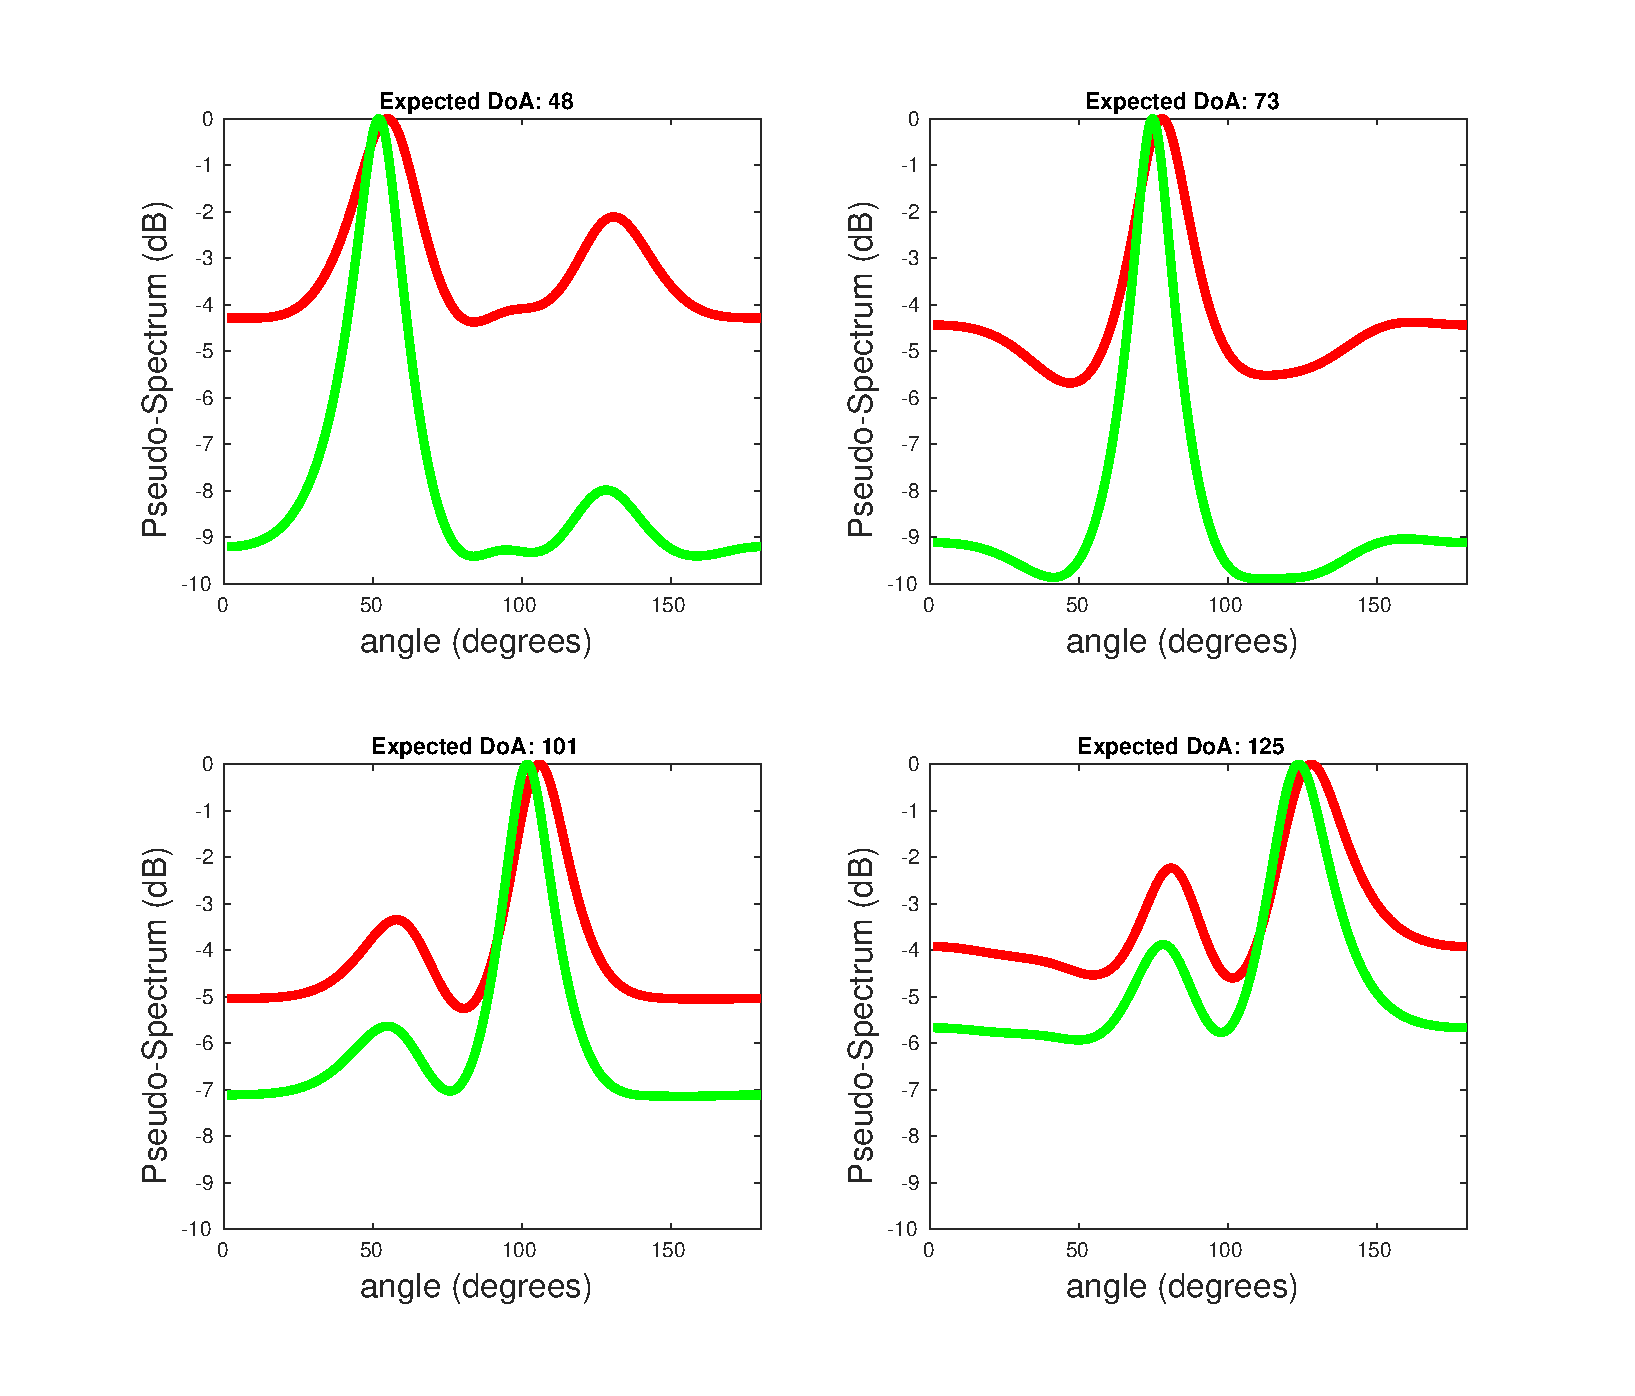
\includegraphics[width=0.85\textwidth]{figures/MUSIC_calib_lin_array_X310_1target.eps}
    \caption{Pseudo-Spectrum of a 1-target DoA Estimation Scenario using \\a Calibrated Linear Array. Experiments Conducted in an Anechoic Chamber.}
    \label{music_x310_calib_lin}
\end{figure}
\begin{figure}[hb!]
    \centering
    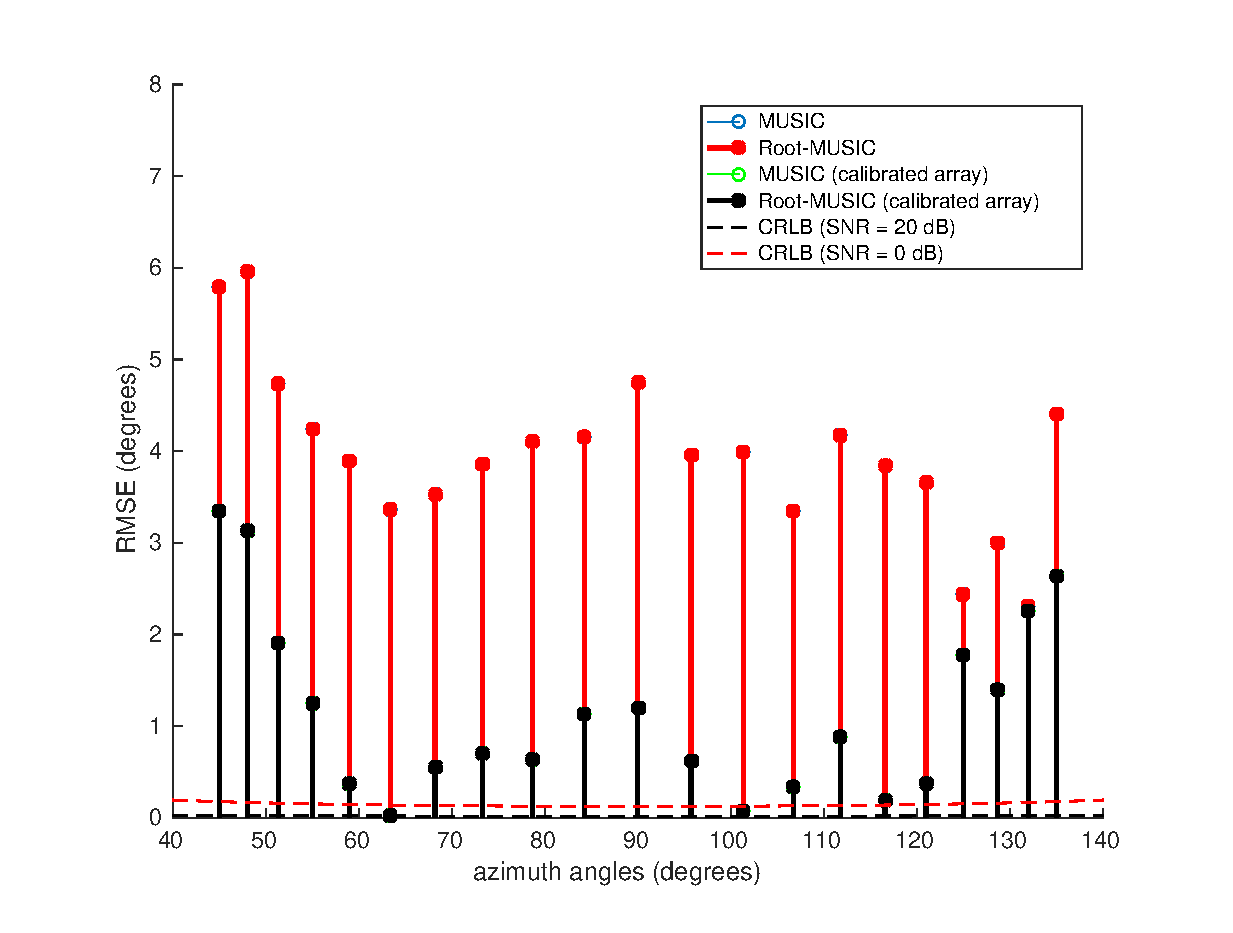
\includegraphics[width=0.67\textwidth]{figures/rmse_calibrated_array.eps}
    \caption{RMSE of MUSIC DoA Estimation using a Linear Array. \\Experiments Conducted in an Anechoic Chamber.}
    \label{RMSE_music_gr}
\end{figure}

To observe the effect of antenna calibration, first navigate to the \texttt{gr-doa/apps} directory and open the flowgraph titled, \texttt{calibrate\_lin\_array\_X310\_TwinRX.grc}. Select appropriate values for the parameters in \texttt{input\_variables}. A screenshot of the this flowgraph is shown in Figure~\ref{calib_lin_array_flowgraph}. Position the transmitter at a known angle and execute this flowgraph to calibrate the antenna array. Then, execute the flowgraph titled, \texttt{run\_MUSIC\_calib\_lin\_array\_X310\_TwinRX.grc} to observe the improvement in the DoA estimated by MUSIC algorithm. As shown in Figure~\ref{music_x310_calib_lin}, we noticed not only an improvement in the SNR of the pseudo-spectrum and a general sharpening of the peak around the true DoA but also an apparent shift of the peak towards the true DoA. This overall improvement in the estimation performance is further illustrated by Figure~\ref{RMSE_music_gr}. The dashed lines in this figure represent the Cramer-Rao Lower Bound as reported in~\cite{stoica1989}. 
\begin{figure}[ht!]
    \centering
    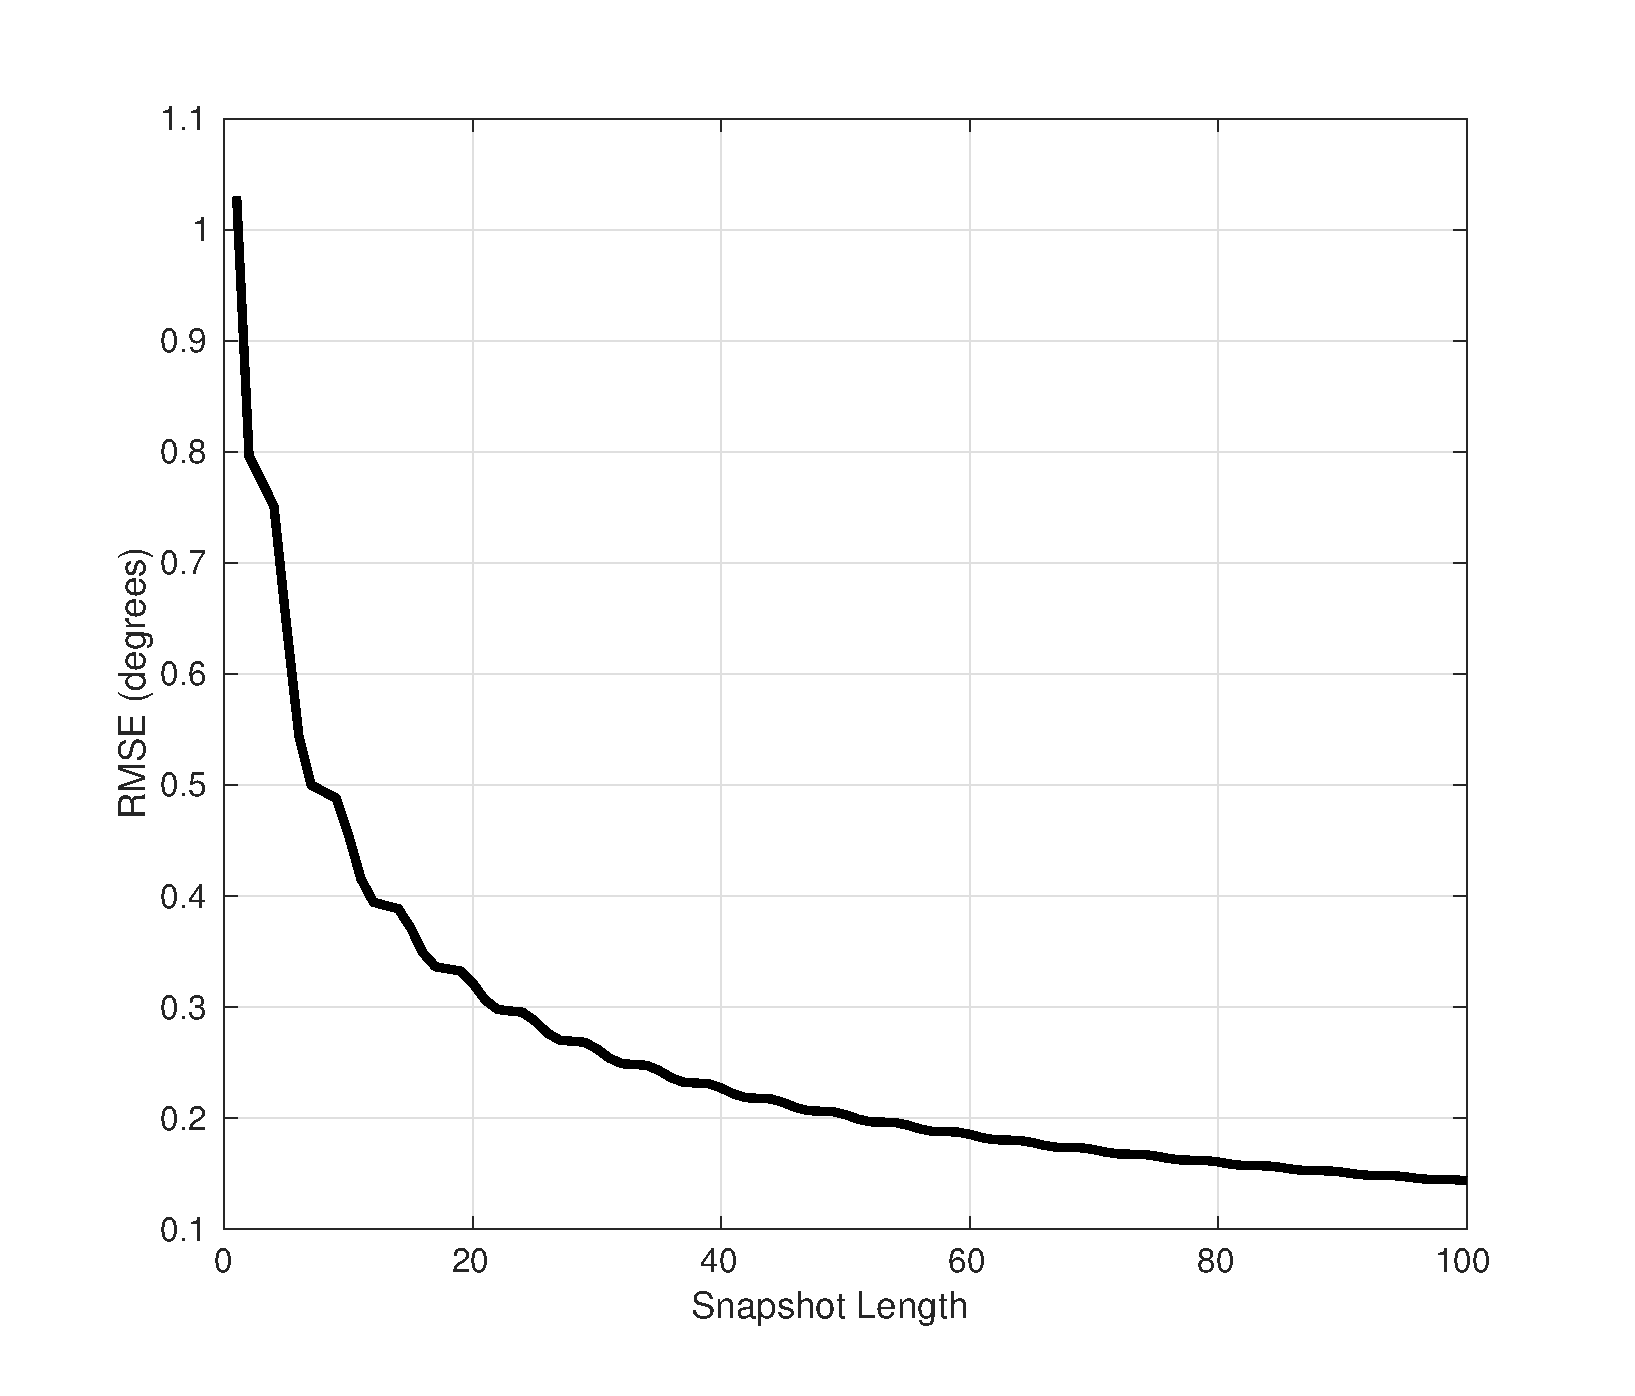
\includegraphics[width=0.7\textwidth]{figures/ss_len_rmse.eps}
    \caption{RMSE of MUSIC DoA Estimation as a Function of Snapshot Length.}
    \label{music_sim_ss}
\end{figure}

\subsection*{Benchmark Tests}
In order to determine the fastest rate at which data can be streamed from an X310 to a host PC to run our DoA implementation, we first conducted a preliminary simulation-based study to understand the effect of \textit{Snapshot Size} parameter on estimation performance. As shown in Figure~\ref{music_sim_ss}, we noticed that the root-mean-squared error (RMSE) progressively decays with increasing snapshot size. As a consequence, we were encouraged to use a sufficiently large value for this parameter such that not only does it help in achieving a reasonable amount of spatial averaging effect when computing the \textit{sample} autocorrelation matrix, but also reduces the RMSE in DoA estimation.

The fundamental reason for focusing on the \texttt{Autocorrelate} block and using its performance as an indicator of the fastest overall rate is due to its computationally-intensive nature. Furthermore, all other operations are performed downstream from the perspective of this \textit{rate-conversion} block except for the \texttt{Phase Correct} block. Hence, this block acts as a rate-limiting block for all practical purposes. In other words, while it can be argued that one of the downstream blocks, such as \texttt{MUSIC}, might operate at a slower rate than \texttt{Autocorrelate} for smaller snapshot sizes and consequently, when more items are made available in the output buffer of \texttt{Autocorrelate} block, smaller snapshot sizes defeat the purpose of accurate DoA estimation as demonstrated by Figure~\ref{music_sim_ss}.

In our experiments, we used both a laptop and a desktop computer acting as the host PC for DoA estimation. The laptop consisted of $8$-cores running at a clock frequency of $1.87$~GHz whereas the desktop machine is a $48$-core computer with a clock frequency of $2.6$~GHz. With the laptop connected to the X310 over a $1$~Gigabit Ethernet interface, we were able to operate at the fastest possible rate, \textit{i.e.,} $6.25$~MS/s per stream without buffer overflow except for snapshot sizes of $32$ and below. With the desktop machine acting as the host PC and with a $1$~Gigabit Ethernet link as the interface, we achieved the fastest possible rate, \textit{i.e.,} $6.25$~MS/s per stream, for smaller snapshot sizes also. 

Our results when the desktop computer was connected to the X310 over a $10$~Gigabit Ethernet interface are shown in Table~\ref{benchmark_table_10gige_desktop}. This table is generated by letting the \texttt{Autocorrelate} block process incoming receive samples for a period of $30$~seconds and then accessing the \texttt{overflow} flag set by the \texttt{top block}. As shown by this table, the fastest possible rate at which we were able to operate was $12.5$~MS/s. Importantly, even at this rate, if the selected snapshot size is too small (or, if it is exceedingly high), the penalty imposed for performing a computationally intense matrix-matrix multiply several times is the inability to keep up with the incoming samples, resulting in buffer overflow. 
\begin{table}[t]
\caption{Occurrence of Buffer Overflow over a $10$~GigE Link.}
\begin{center}
\begin{tabular}{|c|c|c|c|c|c|c|c|c|}
\cline{1-9}
Snapshot & \multicolumn{8}{|c|}{Sample Rate Per Stream (MS/s)} \\
\cline{2-9}
Length& 50 & 25 & 16.67 & 12.5 & 10 & 8.33 & 7.14 & 6.25 \\
\hline
\multicolumn{1}{|c|}{32} & True & True & True & True & True & False & False & False\\
\multicolumn{1}{|c|}{64} & True & True & True & True & False & False & False & False\\
\multicolumn{1}{|c|}{128} & True & True & True & False & False & False & False & False\\
\multicolumn{1}{|c|}{256} & True & True & True & False & False & False & False & False\\
\multicolumn{1}{|c|}{512} & True & True & True & False & False & False & False & False\\
\multicolumn{1}{|c|}{1024} & True & True & True & False & False & False & False & False\\
\multicolumn{1}{|c|}{2048} & True & True & True & False & False & False & False & False\\
\multicolumn{1}{|c|}{4096} & True & True & True & True & False & False & False & False\\
\hline
\end{tabular}
\end{center}
\label{benchmark_table_10gige_desktop}
\end{table}

\section*{\underline{Conclusion}}
This article discusses the phase synchronization feature available by using TwinRX daughterboards. Using a simple calibration procedure, we showed a way to measure and save the fixed repeatable relative phase offsets. Any user-developed software running on the host PC that requires accurate phase synchronization will need to incorporate a phase offset correction step, as we demonstrated in the case of MUSIC-based DoA estimation. The physical experimental results we provided illustrate the performance observed using our lab setup. 

\begin{thebibliography}{9}
\bibitem{pandeya} Neel Pandeya, Nate Temple \emph{Synchronization and MIMO Capability with USRP Devices}. Available from World Wide Web: (\url{https://kb.ettus.com/Synchronization_and_MIMO_Capability_with_USRP_Devices}).
\bibitem{trees} Harry L. Van Trees, "Optimum Array Processing: Part IV of Detection, Estimation, and Modulation Theory", Wiley-Interscience, New York, 2002.
\bibitem{soon1994} V. C. Soon, L. Tong, Y. F. Huang and R. Liu, "A Subspace Method for Estimating Sensor Gains and Phases," in IEEE Transactions on Signal Processing, vol. 42, no. 4, pp. 973-976, Apr 1994.
\bibitem{stoica1989} P. Stoica and A. Nehorai, "MUSIC, Maximum Likelihood, and Cramer-Rao Bound," in IEEE Transactions on Acoustics, Speech, and Signal Processing, vol. 37, no. 5, pp. 720-741, May 1989.
\end{thebibliography}

\end{document}
